% !TeX spellcheck = fr_FR
\chapter{Chapitre 3 : Résultats}

Dans ce chapitre, je vais montrer les résultats que j'ai obtenus des différents implémentations qui ont été faite au chapitre précèdent.  

\section{Bcrypt cracker}

Jusqu'à présent, le système d'attaque n'a été testé seulement à l'aide de simulation. 
Après validation des différents modules à l'aide des testbenchs, j'ai par la suite implémenté le système sur une carte \gls{fpga}.

Pour les tests, j'ai utilisé une Nexys Video qui est la carte \gls{fpga} que l'on utilise durant nos cours.

\begin{figure}[tbph!]
	\centering
	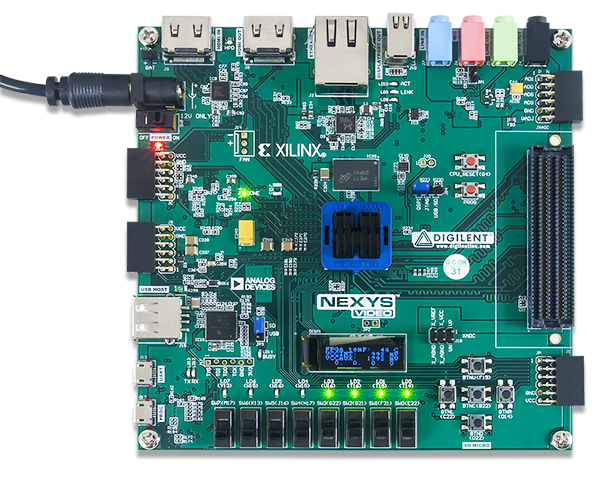
\includegraphics[width=0.9\linewidth]{nexys_video}
	\caption[Carte de développement Nexys Video]{Carte de développement Nexys Video. Source : digilent.com ref. URL02}
	\label{fig:nexys_video}
\end{figure}

\subsection{Validation}

Afin de le tester sur une carte, j'ai tout d'abord fixé dans le code le salt et le hash du mot de passe que l'on souhaite retrouver.
J'ai ensuite connecté les ports \textit{done} et \textit{success} du module sur des LEDS, comme ca lorsque le mot de passe est trouvé, les deux LEDS s'allumeront.
J'ai aussi fait en sortie d'allumer une LED, lorsque le système va démarrer.

\begin{figure}[tbph!]
	\centering
	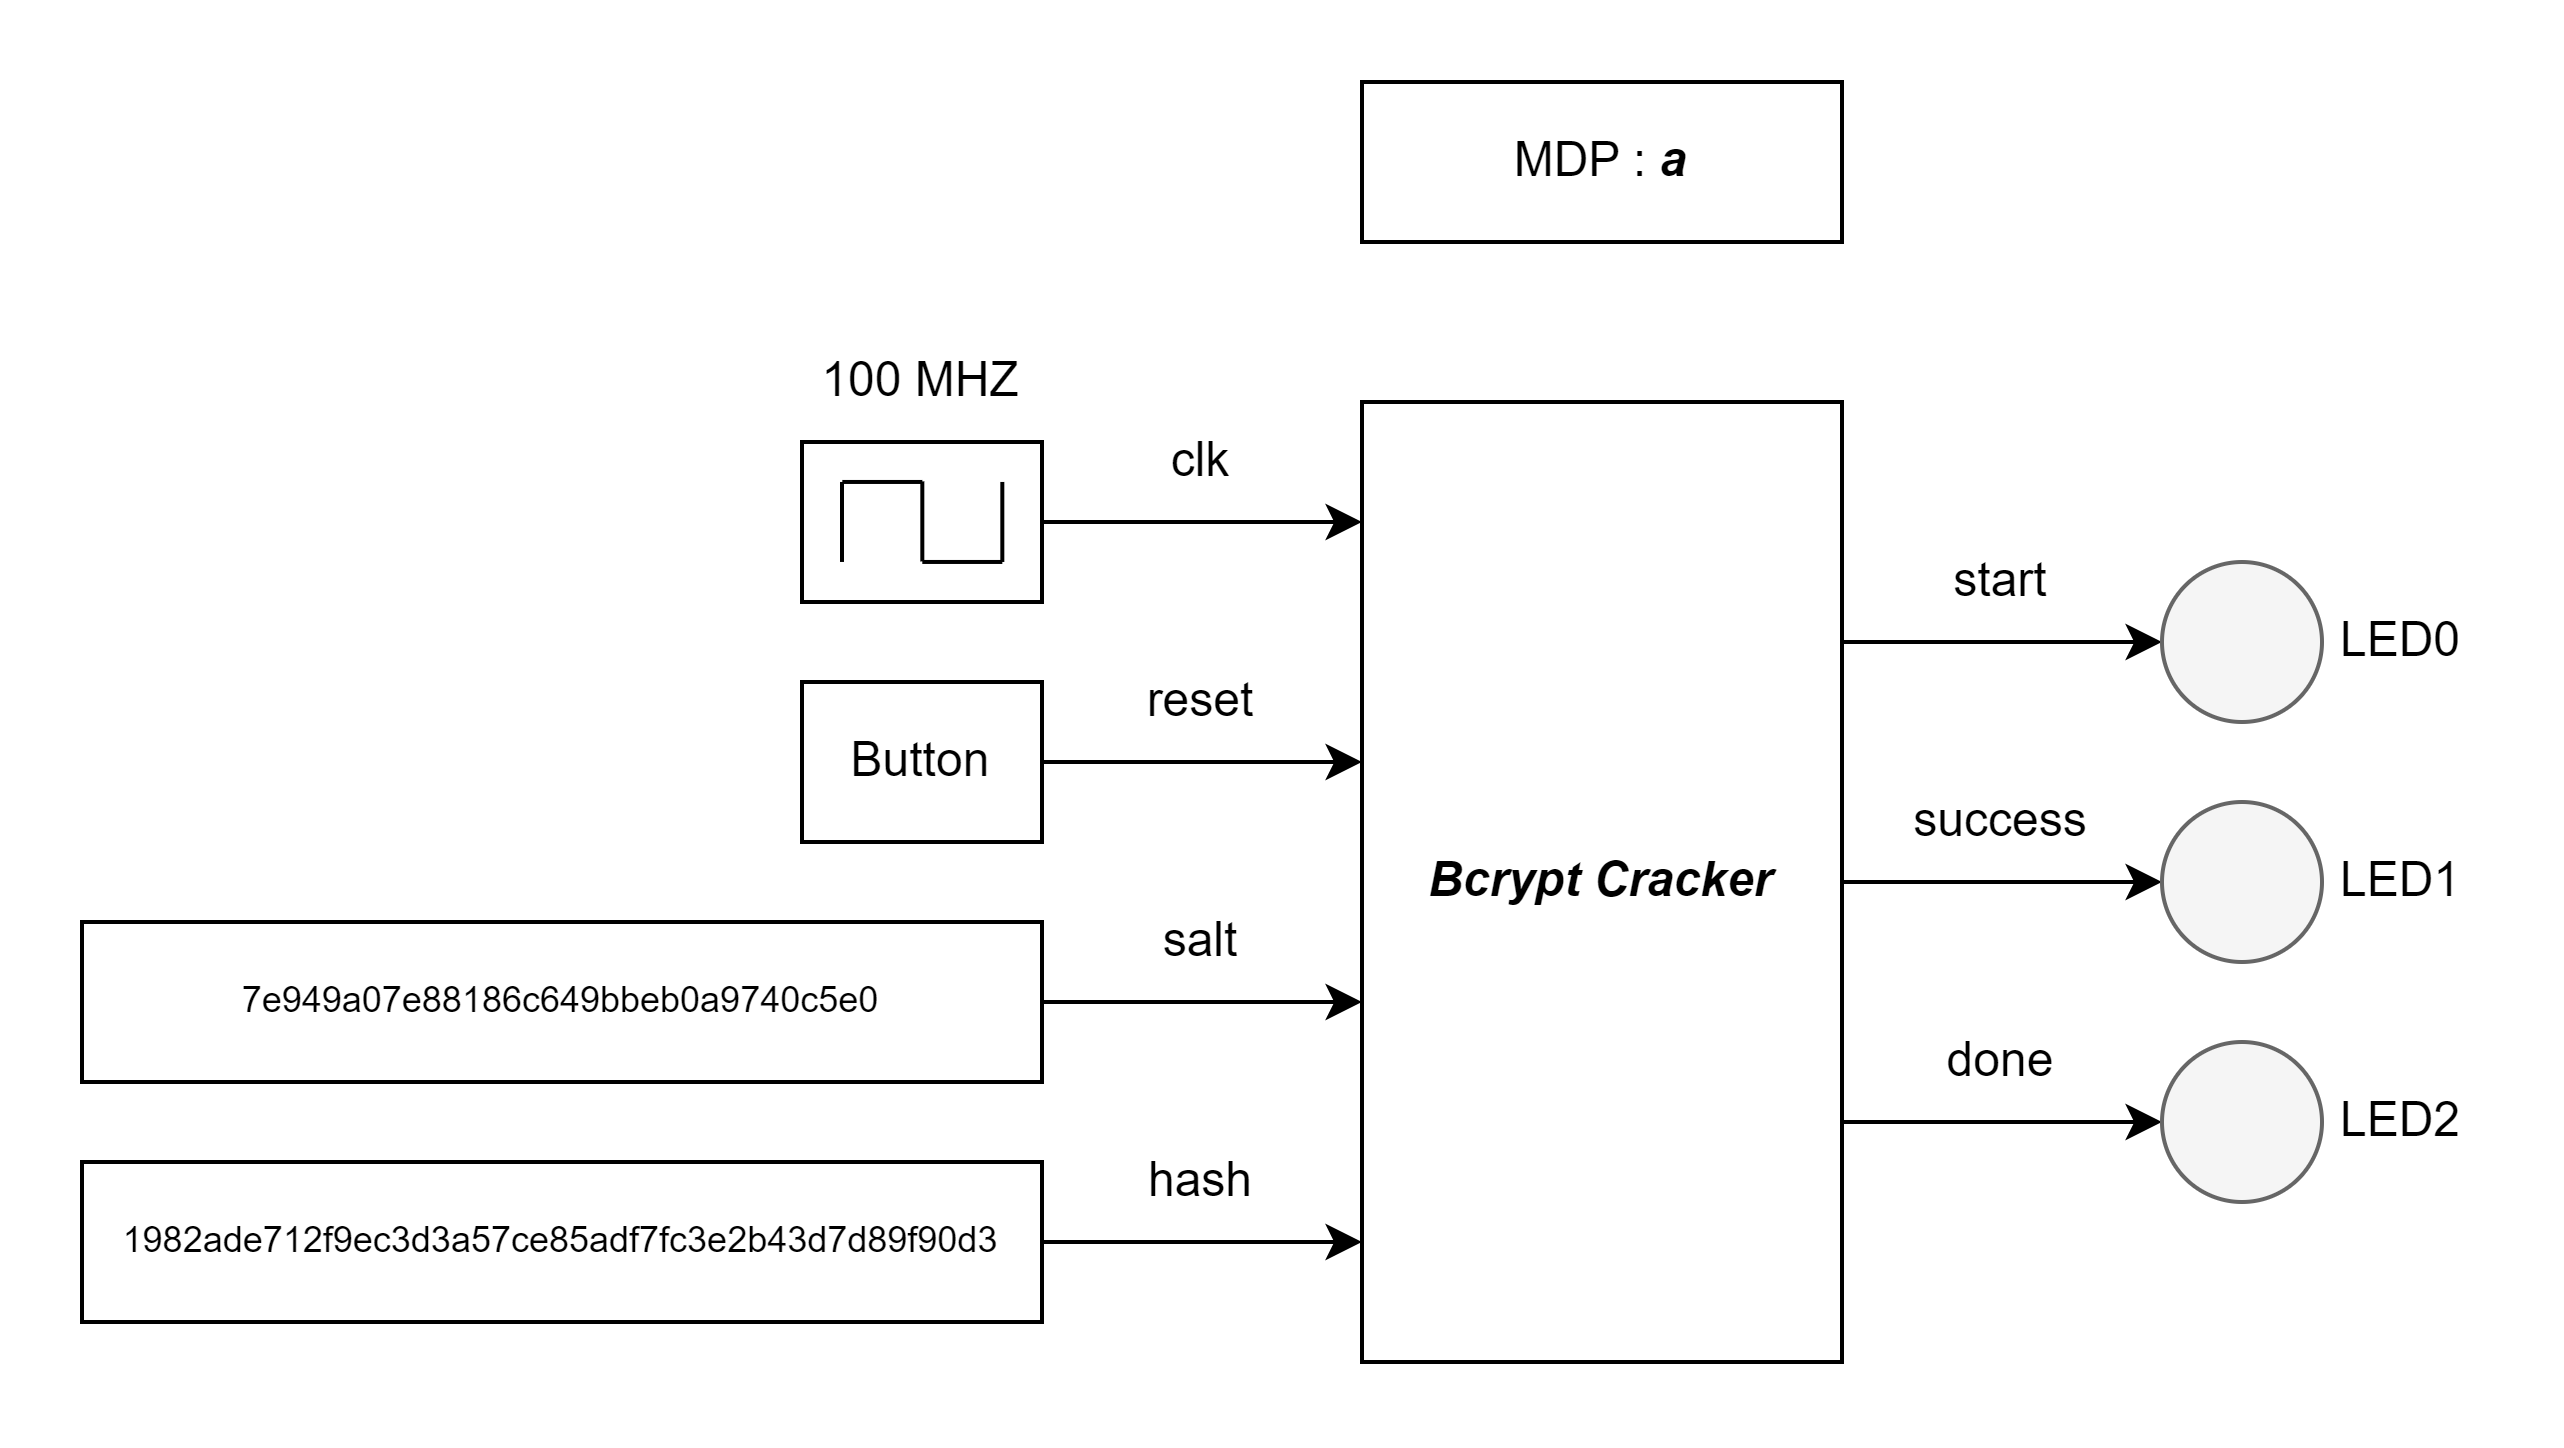
\includegraphics[width=0.7\linewidth]{test_cracker}
	\caption[Schéma du test sur carte]{Schéma du test sur carte. Source : réalisé par Kandiah Abivarman}
	\label{fig:test_cracker}
\end{figure}

Au premier essai, le système ne fonctionnait pas. En effet, les LEDS \textit{start} et \textit{done} se sont bien allumé mais la LED \textit{success} ne s'est pas allumé.
Cela veut dire que le système s'est arréter sans trouver, après avoir atteint le nombre maximale d'essai.

J'ai passé un certain temps à debugger, mais je n'arrivais pas à trouver le problème. 
J'avais néanmoins une piste, un warning me prévenant que certains de mes \gls{bram} étaient retirer lors de la synthèse car inutile. 
Les \gls{bram} qui ont été retiré sont ceux qui sont utilisés pour stocker les valeurs initial des clés de chiffrement.
Ces \gls{bram} sont initialisé à l'aide de fichier dans laquelle sont stockés les decimales de PI, cette méthode était initialement utilisé pour éviter de polluer visuellement le code.
Après conseil de mon professeur, j'ai enlever l'initialisation par fichier externe et j'ai tout simplement mis les valeurs directement dans le code.

J'ai ensuite pu retesté et cette fois-ci le programme a bien fonctionné, les trois LEDS se sont bien allumés.

\newpage

\subsection{Mesures}

A l'aide d'un compteur que j'ai mis en place dans mes testbenchs, j'ai pu observer qu'il faut 649'225 coups d'horloge pour hacher un mot de passe avec un cost de 5.
Le système tourne à 100 MHz, de ce fait le hachage de un mot de passe prend environ 6.49 ms, on arrive donc avec seulement un bcrypt core à un taux de hash par seconde de 154.

Dans Vivado, il est possible de récuperer les ressources utilisés par notre programme dans le \gls{fpga} : 

\begin{figure}[tbph!]
	\centering
	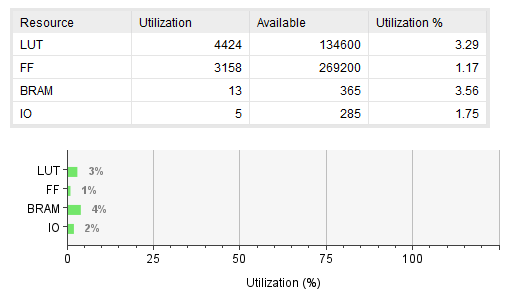
\includegraphics[width=0.7\linewidth]{ressources_usages_cracker_nexys}
	\caption[Ressources utilisés par le bcrypt cracker sur la Nexys Video]{Ressources utilisés par le bcrypt cracker sur la Nexys Video. Source : réalisé par Kandiah Abivarman}
	\label{fig:ressources_usages_cracker_nexys}
\end{figure}

Dans ce programme, j'ai instantié seulement un quadcore dans mon système. On peut voir que la ressource la plus utilisée est la \gls{bram} à hauteur de 3.56\%. 
Avec les ressources disponibles, il serait donc potentiellement possible d'instantier 35 quadcore dans ce système.

Donc avec 35 quadcore, c'est à dire 140 bcrypt core, on arrive à 21'564 hash par seconde. 
A titre de comparaison, un GPU tel que le Nvida RTX-2080Ti qui est un \gls{gpu} haut de gamme a environ 28'000 hash par seconde\footnote{TO DO : ADD LINK}.
Notre résultat est donc assez proche des performances sur \gls{gpu}.

\newpage

\section{Interface PCIe}

Cette partie consiste à montrer comment j'ai pu confirmer le bon fonctionnement de l'interface \gls{pcie} entre une carte \gls{fpga} et un \gls{pc}.

\subsection{Validation}

Pour ce faire, après programmation de la carte, j'ai branché la carte au \gls{pc} puis j'ai lancé la commande linux \textit{lspci} qui est une commande permettant d'afficher des informations
concernant les périphériques \gls{pcie} qui sont connectés.

\begin{figure}[tbph!]
	\centering
	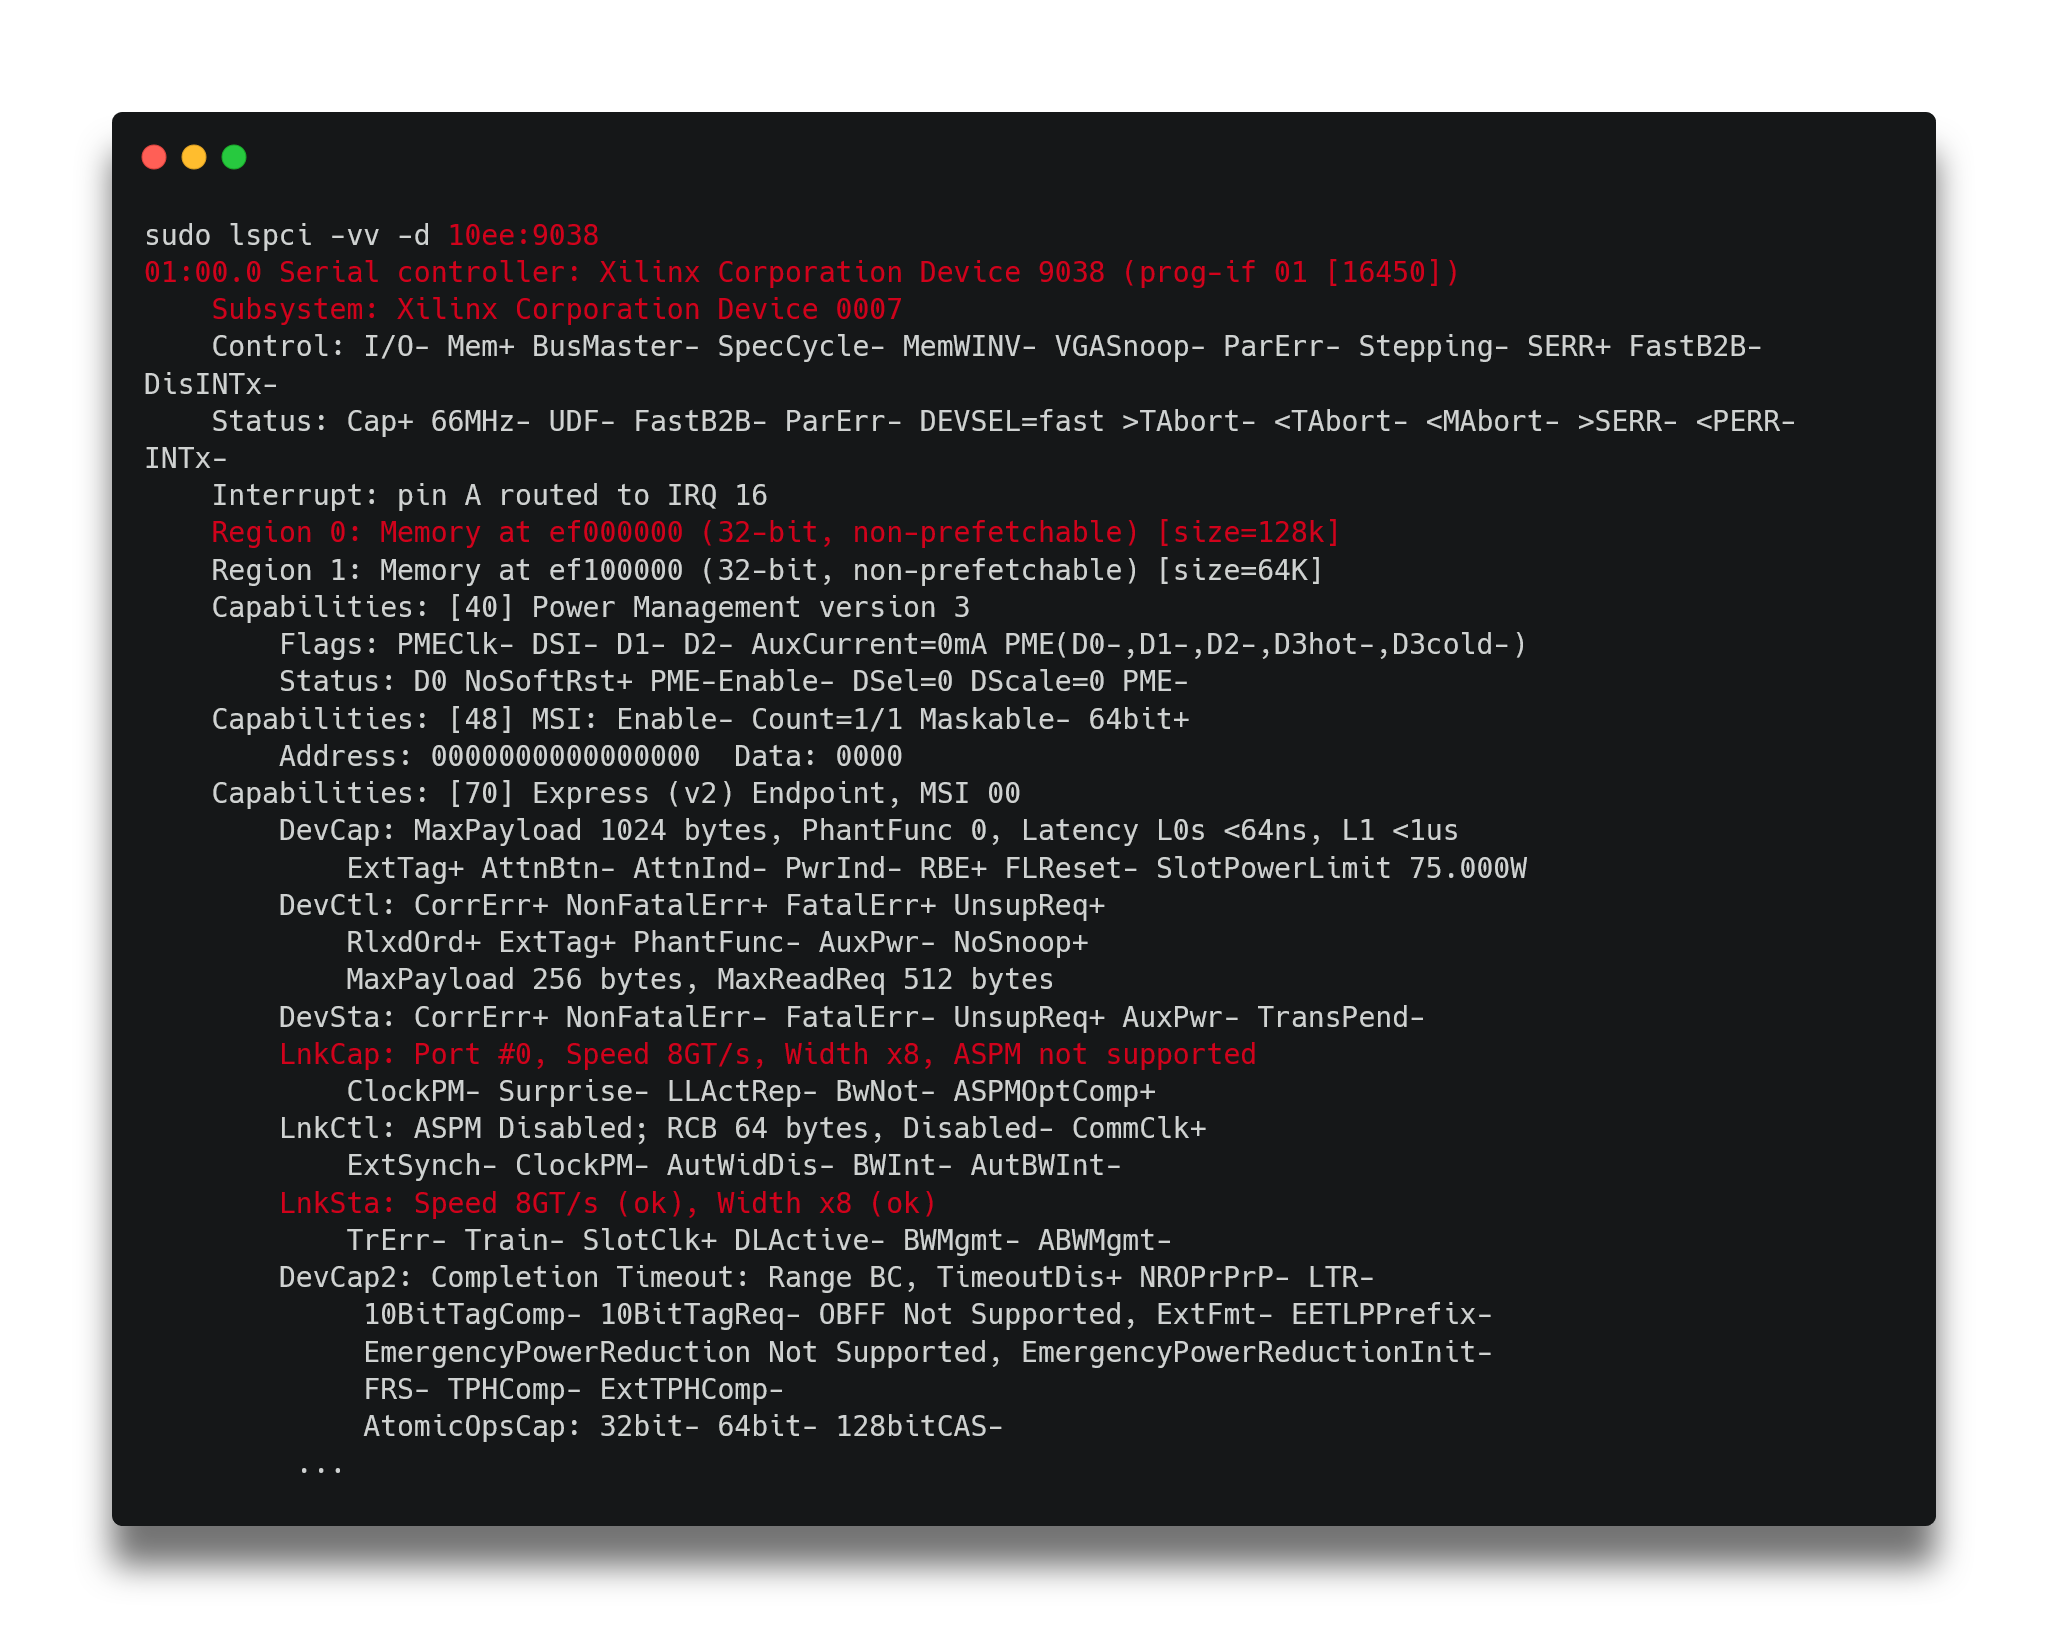
\includegraphics[width=0.7\linewidth]{lspci}
	\caption[lspci pour observer notre carte FPGA]{lspci pour observer notre carte fpga. Source : réalisé par Kandiah Abivarman}
	\label{fig:lspci}
\end{figure}

On peut apercevoir en rouge les différents paramètres que j'ai pu regler dans le chapitre précèdent.

A l'aide de sysfs qui est un système de fichier linux qui permet d'interfacer directement avec les différents périphériques connectés.
TO DO TALK ABOUT SYSFS AND TEST